\section{Models}

In this project, different architectures are used, all based on Convolutional Neural Networks (CNNs) to 
delegate feature extraction to the model, directly using the environment floorplan image as input. Three
distinct models were used:
\begin{enumerate}
    \item AlexNet \cite{NIPS2012_c399862d}, one of the first successful architectures in the field of CNNs;
    \item MobileNetV3 \cite{howard2019searchingmobilenetv3}, the state of the art of
        lightweight CNN architectures designed for mobile and embedded vision applications;
    \item SqueezeNetV2 \cite{iandola2016squeezenetalexnetlevelaccuracy50x}, an ultra-compact CNN with 
        few parameters, offering decent accuracy for low-memory device;
\end{enumerate}

\noindent
Formally, the model $h$ we aim to learn can be expressed as follows:
$$ h: [0,255]^{n\times n} \times \mathbb{R}^+ \rightarrow \mathbb{R}^2 $$
where $[0,255]^{n\times n}$ is a floorplan image encoded as an $n\times n$ grayscale image, $\mathbb{R}^+$ 
is the area of the floorplan expressed in $m^2$, and $\mathbb{R}^2$ contains ATE ($m$) and ARE ($rad$).



\subsection{AlexNet}
To begin, a model based on AlexNet was chosen, one of the first successful architectures in the field of
convolutional neural networks. AlexNet consists of several convolutional layers followed by fully 
connected layers, using ReLU activations and max-pooling. The relatively large number of layers without 
the use of modern techniques to lighten its computational load, makes this model a deep CNN resulting in
a high number of parameters (\num{37298882}).
The abstract structure is shown on Figure
\ref{fig:AlexNet}.

\begin{figure}[H]
    \vspace{0.5em}
    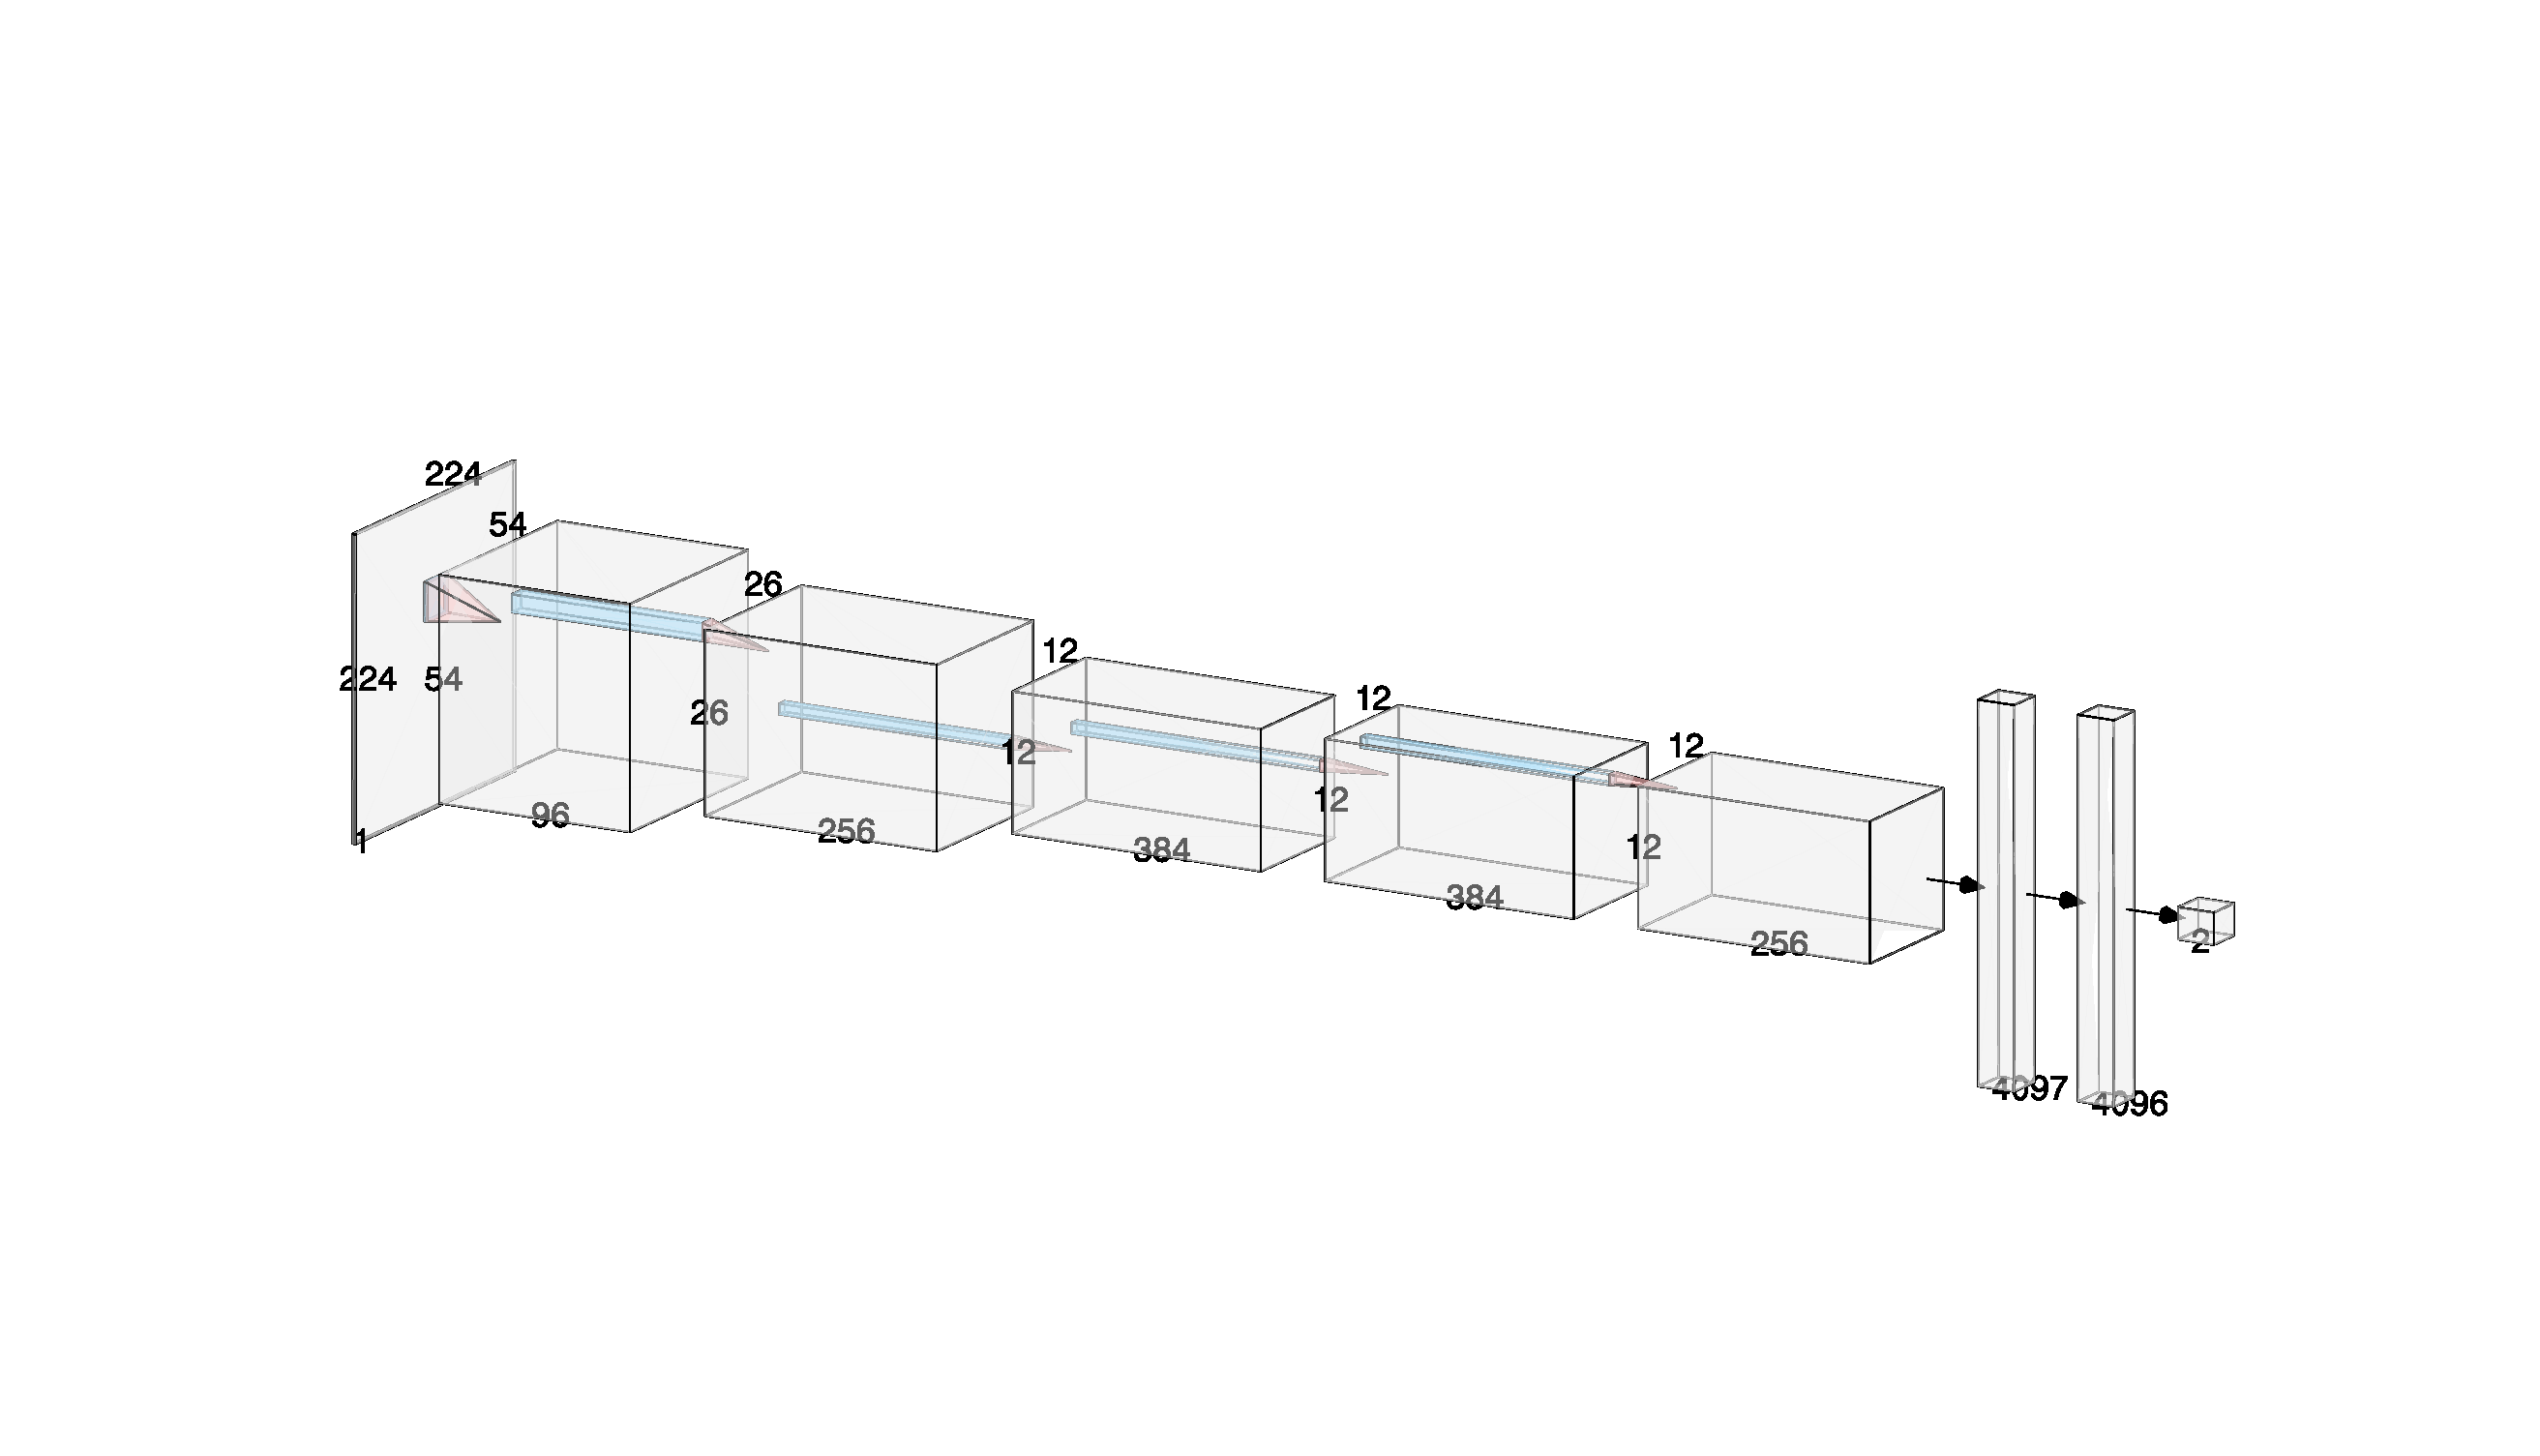
\includegraphics[width=\textwidth,clip, trim=5.9cm 5.8cm 4.5cm 7.5cm]{figures/AlexNet.pdf}
    \caption{Model structure based on AlexNet. Realized with \cite{NNSVG}. \label{fig:AlexNet}}
\end{figure}

\noindent
Two main sections can be outlined: 
\begin{enumerate}
    \item A CNN feature extractor: it processes the input image through a series of convolutional and 
        pooling layers, resulting in a condensed set of features;
    \item A Regression head: it predicts ATE and ARE values through some fully connected layers whose
        input is the set of features extracted from the CNN;
\end{enumerate}

\noindent
Note that the first layer of the regression head has size 4097 instead of 4096, since the area of the 
floorplan is added as an input concatenated to the feature vector extracted by the CNN. This is because
otherwise the scaling done by the model in the initial stage would cause the true value of the area to
be lost.

\subsubsection{Dropout}
To reduce overfitting, the dropout technique \cite{srivastava2014dropout} is applied within the fully
connected layers of the regression head. Dropout randomly sets a fraction of the input units to zero during
training, which prevents the network from relying too heavily on specific features and encourages the 
learning of more robust representations. In our implementation, a dropout rate of 0.5 is used after each
fully connected layer.

\subsection{MobileNetV3}
Despite AlexNet's good accuracy, the computational requirements it needs make it unsuitable for hardware
used in mobile robotics. For this reason, MobileNetV3 was selected as a more efficient alternative, 
offering a state-of-the-art trade-off between accuracy and computational efficiency. In particular, the
MobileNetV3 small version was used, which has \num{1520642} parameters, 24 times less than AlexNet.

To achieve this result, different optimization techniques are used, but we will focus only on the main ones.

\subsubsection{Depthwise and Pointwise Convolutions}
Convolutional layers on which CNNs are based have led to massive achievements in machine learning projects,
especially in computer vision. However, standard convolutions are computationally expensive, particularly
for deep networks. MobileNetV1 addresses this by employing depthwise separable convolutions, which split
the convolution operation into two parts: 
\begin{enumerate}
    \item Depthwise convolution: processes each input channel separately with its own filter, extracting 
    spatial features independently for each channel;
    \item Pointwise convolution: applies $1\times1$ convolutions across all channels, combining the outputs
    from the depthwise step to integrate information across channels;
\end{enumerate}

\begin{figure}[H]
    \centering
    \vspace{-1em}
    \begin{minipage}{0.46\textwidth}
        \centering
        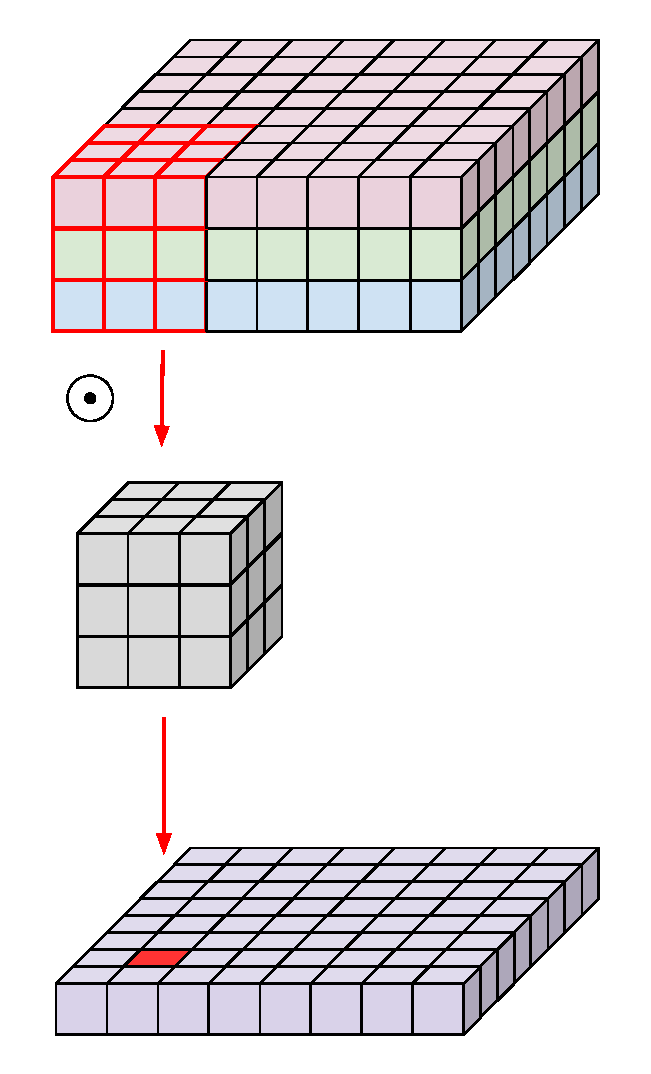
\includegraphics[width=\textwidth]{figures/conv2d-3d.pdf}
    \end{minipage}\hfill
    \begin{minipage}{0.5\textwidth}
        \centering \vspace{-.1em}
        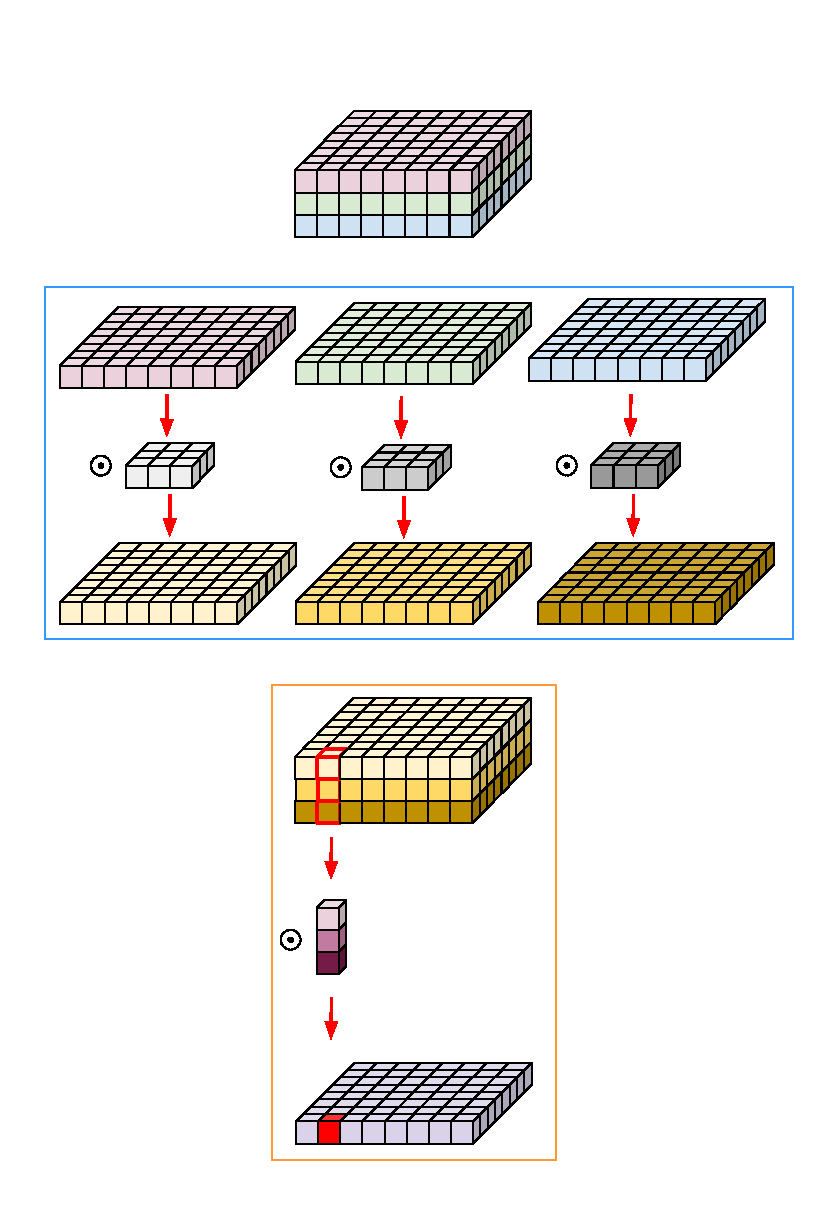
\includegraphics[
            width=\textwidth,clip, trim=0.75cm 1.1cm 0.65cm 2cm
        ]{figures/conv2d-depthwise-separable.pdf}
    \end{minipage}
    \vspace{-1em}
    \captionsetup{width=0.95\linewidth}
    \caption{Standard Convolution (left) and Deepthwise+Pointwise Convolution (right).
    The Deepthwise conv. is highlighted in light blue while Pointwise conv. in orange
    \cite{depthwiseConv}.}
\end{figure}

\noindent
To understand computational savings, take the follwing example: let $S$ be the dimensions of the squared 
input, $K$ the dimensions of the squared kernel filter, $C_{in}$ the number of input channels and $C_{out}$
the numbers of output channels. We'll assume:
$$\begin{matrix}
    S=128 & K=3 \ & C_{in}=3 \ & C_{out}=16
\end{matrix}$$ \vspace{-2em}
\begin{table}[H]
    \centering
    \begin{tabular}{|c|c|c|} \hline
    & Regular convolution & Deepthwise and Pointwise convolution \\ \hline
    Parameters & $3^2\cdot3\cdot16=432$ & $3^2\cdot3\cdot128^2\cdot16=\num{7077888}$ \\
    \# multiplications & $3^2\cdot3+3\cdot16=75$ & $3^2\cdot3\cdot128^2+128^2\cdot3\cdot16=\num{1228800}$ \\
    \hline
    \end{tabular}
\end{table}

\subsubsection{Squeeze and Excitation}
Introduced in \cite{hu2019squeezeandexcitationnetworks}, Squeeze and Excitation is a technique that focuses on
the interdependencies between channels. As the name suggests, there are two phases:
\begin{enumerate}
    \item Squeeze phase: each channel is squeezed into a single value through the use of averge pooling.
        The output of this phase is then a vector $\bm{z}$ of $C$ elements, where $C$ is the number of channels:
        $$ \bm{z} =\{z_1,\dots,z_C\} $$
        \begin{equation}
            z_c = \frac{1}{HW}\sum_{i=1}^{H}\sum_{j=1}^{W}u_c(i,j) \tag*{c=1,\dots,C}
        \end{equation}
        where $\bm{U}=\{\bm{u}_1,\dots,\bm{u}_C\}$ is the set of feature maps of size $H\times W$ and
         $u_c(i,j)$ is the element in position $(i,j)$ on the $c$-th feature map.
    \item Excitation phase: the squeezed vector $\bm{z}$ is fed into a two-layer feed-forward neural network
        composed of a first layer of size $C/r$ with ReLU and a second layer of size $C$ with sigmoid, where
        $\text{sigmoid}(x)= 1/(1+e^{-x})$ and $r$ is a reduction ratio.
        The purpose of this phase is to capture the intricate dependencies among channels. The output of this 
        network is another vector $\bm{s}$ of the same dimensions of $\bm{z}$, containing the importance 
        weights for each channel.
    \item Scale and combine phase: the importance weights vector $\bm{s}$ is used to rescale each channel of the 
        original input by channel-wise multiplication ($*$):
        \begin{equation}
        \tilde{\bm{x}}_c = s_c * \bm{u}_c   \tag*{c=1,\dots,C}
        \end{equation}
        where $\tilde{\bm{X}} = \{\tilde{\bm{x}}_1,\dots,\tilde{\bm{x}}_C\}$ is the final output.
\end{enumerate}

\begin{figure}[H]
    \centering
    \resizebox{\textwidth}{!}{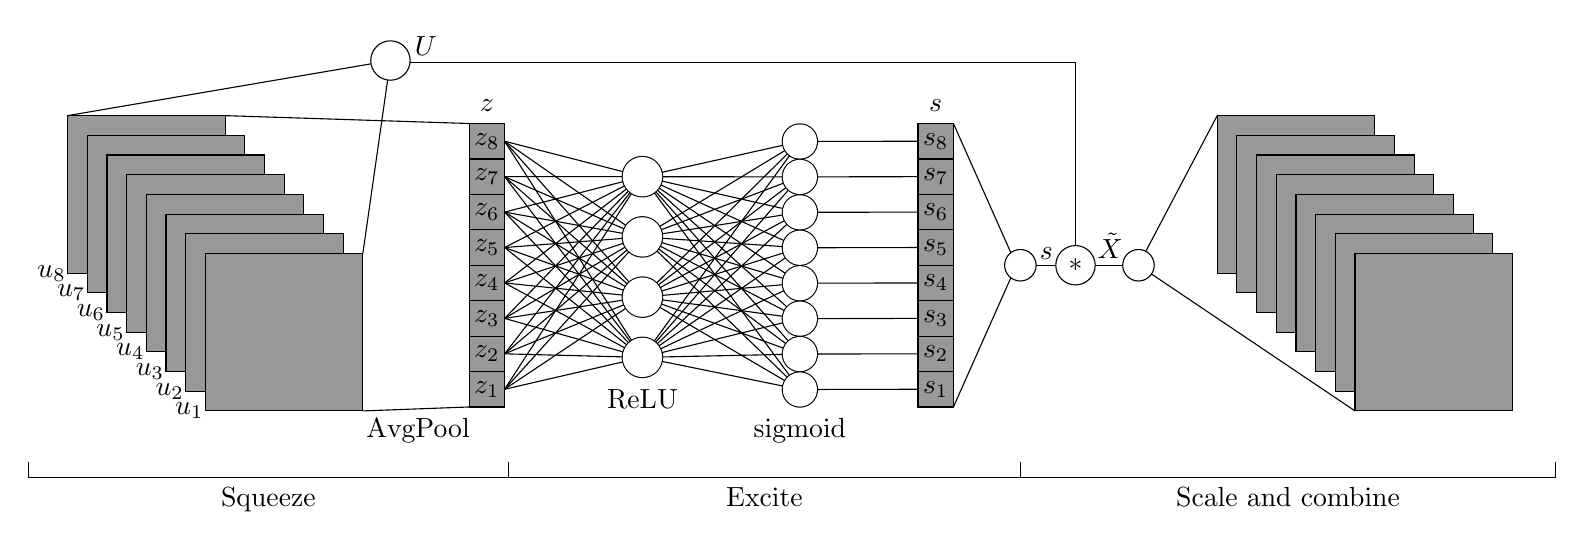
\begin{tikzpicture}

    \definecolor{color1}{HTML}{1f77b4}   % blue
    \definecolor{color2}{HTML}{ff7f0e}   % orange
    \definecolor{color3}{HTML}{2ca02c}   % green
    \definecolor{color4}{HTML}{d62728}   % red
    \definecolor{color5}{HTML}{9467bd}   % purple
    \definecolor{color6}{HTML}{8c564b}   % brown
    \definecolor{color7}{HTML}{e377c2}   % pink
    \definecolor{color8}{HTML}{bcbd22}   % olive
    
    \colorlet{case}{black}
    
    \newcommand{\setColor}[1]{
        \ifthenelse{#1=0}{\colorlet{case}{color1}}{}
        \ifthenelse{#1=1}{\colorlet{case}{color2}}{}
        \ifthenelse{#1=2}{\colorlet{case}{color3}}{}
        \ifthenelse{#1=3}{\colorlet{case}{color4}}{}
        \ifthenelse{#1=4}{\colorlet{case}{color5}}{}
        \ifthenelse{#1=5}{\colorlet{case}{color6}}{}
        \ifthenelse{#1=6}{\colorlet{case}{color7}}{}
        \ifthenelse{#1=7}{\colorlet{case}{color8}}{}
    }

    %\foreach \y in {-2,-1.9,...,4} {
    %    \draw [color=black!20] (-1,\y) -- (12,\y);
    %}

    \def\offsetx{-0.6}
    \def\offsety{+0.5}
    \foreach \x / \i in {0/7,0.25/6,0.5/5,0.75/4,1/3,1.25/2,1.5/1,1.75/0} {
        \pgfmathtruncatemacro{\y}{\i+1}
        \setColor{\i}
        \draw [fill=case!40] (-0.7+\x+\offsetx,0.7-\x+\offsety) rectangle 
            (1.3+\x+\offsetx,2.7-\x+\offsety);
        \node [left] at (-0.6+\x+\offsetx,0.7-\x+\offsety) {$\bm{u}_\y$};
    }

    \def\d{0.45}
    \pgfplotsforeachungrouped \x / \y in {0/1,1/2,2/3,3/4,4/5,5/6,6/7,7/8} {
        \setColor{\x}
        \draw [fill=case!40] (3.8,-0.5+\x*\d) rectangle (3.8+\d,-0.5+\d+\x*\d);
        \node at (3.8+\d/2,-0.5+\x*\d+\d/2) {$z_{\y}$};
    }
    \node at (3.15,-0.8) {AvgPool};
    \node at (3.8+\d/2,-0.5+8*\d+\d/2) {$\bm{z}$};

    \draw (1.3+1.75+\offsetx,0.7-1.75+\offsety) -- (3.8,-0.5);
    \draw (1.3+\offsetx,2.7+\offsety) -- (3.8,-0.5+\d+7*\d);

    \foreach \x in {0,1,...,3} {
        \foreach \y in {0,...,7} {
            \draw (3.8+\d,-0.5+\y*\d+\d/2) -- (6,0.13+\d*1.7*\x);
        }
        \draw[color=black,thick] (6,0.13+\d*1.7*\x) circle [radius=0.25];
    }
    \node at (6,-0.4) {ReLU};
    \foreach \x in {0,1,...,7} {
        \foreach \y in {0,...,3} {
            \draw (6,0.13+\y*\d*1.7) -- (8,-0.278+\d*\x);
        }
        \draw[color=black,thick] (8,-0.278+\d*\x) circle [radius=0.217];
    }
    \node at (8,-0.8) {sigmoid};
    \foreach \x/\y in {0/1,1/2,2/3,3/4,4/5,5/6,6/7,7/8} {
        \draw (8,-0.278+\d*\x) -- (9.5,-0.5+\x*\d+\d/2);
        \setColor{\x}
        \draw [fill=case!40] (9.5,-0.5+\x*\d) rectangle (9.5+\d,-0.5+\d+\x*\d);
        \node at (9.5+\d/2,-0.5+\x*\d+\d/2) {$s_\y$};
    }
    \node at (9.5+\d/2,-0.5+8*\d+\d/2) {$\bm{s}$};
    \foreach \x in {0,1,...,3} {
        \fill[color=white] (6,0.13+\d*1.7*\x) circle [radius=0.25];
    }
    \foreach \x in {0,1,...,7} {
        \fill[color=white] (8,-0.278+\d*\x) circle [radius=0.217];
    }

    \draw (11.5,1.3) circle [radius=0.25];
    \node at (11.5,1.3) {$*$};
    \draw (9.5+\d,-0.5)         -- (11-0.25,1.3);
    \draw (9.5+\d,-0.5+\d+7*\d) -- (11-0.25,1.3);
    \draw (10.8,1.3) -- (11.5-0.25,1.3);
    \draw [fill=white] (10.8,1.3) circle [radius=0.2];
    \node at (10.8,1.28) {$\shortrightarrow$};

    \foreach \x in {0,0.25,...,1.75}{
        \pgfmathtruncatemacro{\y}{7-\x/0.25}
        \pgfmathtruncatemacro{\i}{\y+1}
        \setColor{\y}
        \draw[fill=case!40] (13.3+\x,2.45-1.75+\offsety-\x) rectangle 
            (15.3+\x,4.45-1.75+\offsety-\x);
    }

    \draw (-0.7+\offsetx,2.7+\offsety) -- (2.8,3.9);
    \draw (1.3+1.75+\offsetx,2.7-1.75+\offsety) -- (2.8,3.9);
    \draw (2.8,3.88) -- (11.5,3.88) -- (11.5,1.3+0.25);
    \draw [fill=white] (2.8,3.9) circle [radius=0.25];
    \node at (3.25,4.08) {$\bm{U}$};
    \node at (2.8,3.88) {$\shortrightarrow$};
    
    \node at (11.13,1.45) {$\bm{s}$};
    \node at (11.94,1.55) {$\tilde{\bm{X}}$};
    \draw (11.5+0.25,1.3) -- (12.2,1.3); 
    \draw (12.3,1.3) -- (13.3,4.45-1.75+\offsety);
    \draw (12.3,1.3) -- (13.3+1.75,2.45-1.75+\offsety-1.75);
    \draw [fill=white] (12.3,1.3) circle [radius=0.2];
    \node at (12.3,1.28) {$\shortrightarrow$};

    \draw (-1.8,-1.2)--(-1.8,-1.4)--(4.3,-1.4)--(4.3,-1.2); 
    \draw (4.3,-1.2)--(4.3,-1.4)--(10.8,-1.4)--(10.8,-1.2); 
    \draw (10.8,-1.2)--(10.8,-1.4)--(17.6,-1.4)--(17.6,-1.2);
    \node [below] at (1.25,-1.4) {Squeeze};
    \node [below] at (7.55,-1.4) {Excite};
    \node [below] at (14.2,-1.4) {Scale and combine};

\end{tikzpicture}}
\end{figure}

\subsubsection{HardSwish Activation function}
To improve the accuracy of the neural networks ReLU was replaced by a new activation function called 
\textit{swish}, defined as:
$$ \text{swish}\ x = x\cdot \sigma(x) $$
where $\sigma$ is the sigmoid function $\sigma(x)=1/(1+e^{-x})$.
However, despite swish improves accuracy, it is computationally expensive for mobile devices. To address this,
MobileNetV3 introduces the \textit{HardSwish} activation function, which approximates swish while being more
efficient to compute. HardSwish is defined as:
$$ \text{\text{h-swish}}(x) = x \cdot \frac{\text{ReLU6}(x + 3)}{6} $$
where $\text{ReLU6}(x) = \min(\max(0, x), 6)$. This function retains the benefits of swish but is faster and
more suitable for deployment on resource-constrained hardware.
\begin{figure}[H]
    \centering
    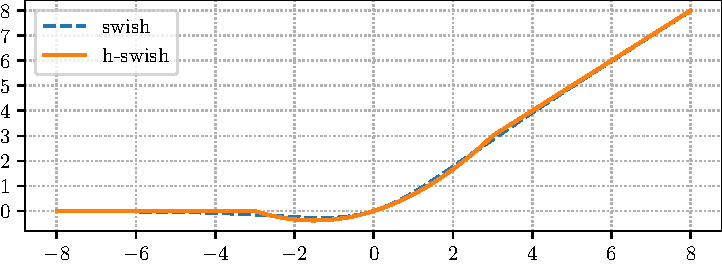
\includegraphics[width=.6\textwidth]{figures/hswish.pdf}
    \caption{Swish and h-swish}
\end{figure}